\documentclass[12pt,letterpaper]{exam}
\usepackage[lmargin=1in,rmargin=1in,tmargin=1in,bmargin=1in]{geometry}
\usepackage{../style/exams}

% -------------------
% Course & Exam Information
% -------------------
\newcommand{\course}{MAT 101: Exam 1}
\newcommand{\term}{Fall -- 2022}
\newcommand{\examdate}{10/07/2022}
\newcommand{\timelimit}{85 Minutes}

\setbool{hideans}{false} % Student: True; Instructor: False

% -------------------
% Content
% -------------------
\begin{document}

\examtitle
\instructions{Write your name on the appropriate line on the exam cover sheet. This exam contains \numpages\ pages (including this cover page) and \numquestions\ questions. Check that you have every page of the exam. Answer the questions in the spaces provided on the question sheets. Be sure to answer every part of each question and show all your work.} 
\scores
%\bottomline
\newpage

% ---------
% Questions
% ---------
\begin{questions}

% Question 1
\newpage
\question[10] Mark each  of the following statements as True ($T$) or False ($F$). \pspace
\begin{enumerate}[(a)]
\item \underline{\itshape\hspace{0.65cm}F\hspace{0.65cm}}: The number 1 is prime. \vfill
\item \underline{\itshape\hspace{0.6cm}T\hspace{0.6cm}}: Every rational number is a real number. \vfill
\item \underline{\itshape\hspace{0.65cm}F\hspace{0.65cm}}: The number $0.5 \cdot 10^{-3}$ is in scientific notation. \vfill
\item \underline{\itshape\hspace{0.65cm}F\hspace{0.65cm}}: Every real number is a rational number. \vfill
\item \underline{\itshape\hspace{0.6cm}T\hspace{0.6cm}}: The number 6 has four positive divisors. \vfill
\item \underline{\itshape\hspace{0.6cm}T\hspace{0.6cm}}: Every integer greater than 1 is either prime or can be written as a product of primes. \vfill
\item \underline{\itshape\hspace{0.6cm}T\hspace{0.6cm}}: $\left( \sqrt[20]{\pi^5} \right)^4= \pi$ \vfill
\item \underline{\itshape\hspace{0.6cm}T\hspace{0.6cm}}: A positive number decreased by 20\% results in the same number as finding 80\% of the number. \vfill
\item \underline{\itshape\hspace{0.65cm}F\hspace{0.65cm}}: All real numbers have a square root that is a real number. \vfill
\item \underline{\itshape\hspace{0.6cm}T\hspace{0.6cm}}: A real number is rational if and only if it has a decimal expansion that repeats. \vfill
\end{enumerate}



% Question 2
\newpage
\question[10] Showing all your work, find the prime factorizations of the following integers---if the integer is prime, simply state this:
	\begin{enumerate}[(a)]
	\item $49$
	\item $54$
	\item $75$
	\item $131$
	\item $621$
	\end{enumerate} \pspace

\sol
\begin{enumerate}[(a)]
\item $49= 7^2$
        	\[
	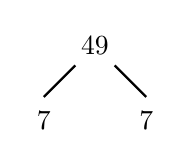
\begin{tikzpicture}
	\node at (-0.15,0.15) {$49$};
	\draw[line width=0.03cm] (-0.4,-0.1) -- (-0.8,-0.5);
	\node at (-0.8,-0.8) {$7$};
	\draw[line width=0.03cm]  (0.1,-0.1) -- (0.5,-0.5);
	\node at (0.5,-0.8) {$7$};
	\end{tikzpicture}
	\] \pspace

\item $54= 2 \cdot 3^3$
        	\[
	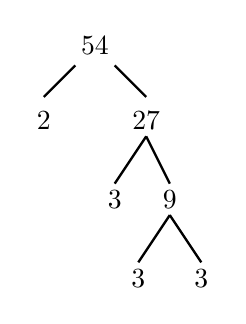
\begin{tikzpicture}
	\node at (-0.15,0.15) {$54$};
	\draw[line width=0.03cm] (-0.4,-0.1) -- (-0.8,-0.5);
	\node at (-0.8,-0.8) {$2$};
	\draw[line width=0.03cm]  (0.1,-0.1) -- (0.5,-0.5);
	\node at (0.5,-0.8) {$27$};
	
	\draw[line width=0.03cm] (0.5,-1) -- (0.1,-1.6);
	\node at (0.1,-1.8) {$3$};
	\draw[line width=0.03cm] (0.5,-1) -- (0.8,-1.6);
	\node at (0.8,-1.8) {$9$};
	\draw[line width=0.03cm] (0.8,-2.0) -- (0.4,-2.6);
	\node at (0.4,-2.8) {$3$};
	\draw[line width=0.03cm] (0.8,-2.0) -- (1.2,-2.6);
	\node at (1.2,-2.8) {$3$};
	\end{tikzpicture}
	\] \pspace

\item $75= 3 \cdot 5^2$
        	\[
	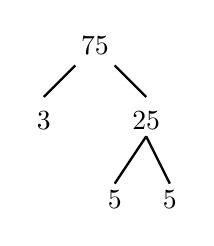
\begin{tikzpicture}
	\node at (-0.15,0.15) {$75$};
	\draw[line width=0.03cm] (-0.4,-0.1) -- (-0.8,-0.5);
	\node at (-0.8,-0.8) {$3$};
	\draw[line width=0.03cm]  (0.1,-0.1) -- (0.5,-0.5);
	\node at (0.5,-0.8) {$25$};
	
	\draw[line width=0.03cm] (0.5,-1) -- (0.1,-1.6);
	\node at (0.1,-1.8) {$5$};
	\draw[line width=0.03cm] (0.5,-1) -- (0.8,-1.6);
	\node at (0.8,-1.8) {$5$};
	\end{tikzpicture}
	\] \pspace

\item 131 is prime, i.e. $131= 131^1$ \pspace

\item $621= 3^3 \cdot 23$
        	\[
	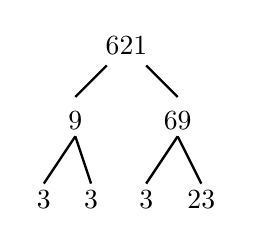
\begin{tikzpicture}
	\node at (-0.15,0.15) {$621$};
	\draw[line width=0.03cm] (-0.4,-0.1) -- (-0.8,-0.5);
	\node at (-0.8,-0.8) {$9$};
	\draw[line width=0.03cm]  (0.1,-0.1) -- (0.5,-0.5);
	\node at (0.5,-0.8) {$69$};
		
	\draw[line width=0.03cm] (-0.8,-1) -- (-1.2,-1.6);
	\node at (-1.2,-1.8) {$3$};
	\draw[line width=0.03cm] (-0.8,-1) -- (-0.6,-1.6);
	\node at (-0.6,-1.8) {$3$};
	
	\draw[line width=0.03cm] (0.5,-1) -- (0.1,-1.6);
	\node at (0.1,-1.8) {$3$};
	\draw[line width=0.03cm] (0.5,-1) -- (0.8,-1.6);
	\node at (0.8,-1.8) {$23$};
	\end{tikzpicture}
	\]
\end{enumerate}



% Question 3
\newpage
\question Without performing any explicit computation, e.g. saying $6/2= 3$ is an integer or $7/2= 3.5$ is not an integer, justify the following statements:
	\begin{parts}
	\part[3] The integer 5,549,787,074,121 is divisible by 3.
	\part[3] The integer 13,513,205,490,217,689,368 is not divisible by 5.
	\part[4] The integer 202,202,022 is divisible by 6.
	\end{parts} \pspace

\sol {\itshape
\begin{enumerate}[(a)]
\item An integer is divisible by 3 if and only if the sum of the digits is divisible by 3. We have\dots
	\[
	5 + 5 + 4 + 9 + 7 + 8 + 7 + 0 + 7 + 4 + 1 + 2 + 1= 60
	\]
Because 60 is divisible by 3, we know that 5,549,787,074,121 divisible by 3. \pspace

\item An integer is divisible by 5 if and only if it ends in 0 or 5. Because the integer 13,513,205,490,217,689,368 does not end in 0 or 5, it is not divisible by 5. \pspace

\item An integer is divisible by 6 if and only if it is divisible by both 2 and 3. An integer is divisible by 2 if and only if it is even. Because 202,202,022 is even, it is divisible by 2. An integer is divisible by 3 if and only if the sum of the digits is divisible by 3. We have $2 + 0 + 2 + 2 + 0 + 2 + 0 + 2 + 2= 12$, which is divisible by 3. But then 202,202,022 is divisible by 3. Because 202,202,022 is divisible by 2 and 3, it is divisible by 6. 
\end{enumerate}
}



% Question 4
\newpage
\question  Showing any necessary work, answer the following:
	\begin{parts}
	\part[3] Find at least three multiples of 12.
	\part[3] Find at least two divisors of 140. 
	\part[4] Find the least common multiple of the smallest and largest prime factor of 30.
	\end{parts} \pspace

\sol {\itshape
\begin{enumerate}[(a)]
\item The multiples of 12 are $0, 12, 24, 36, 48, 60, \ldots$ and $-12, -24, -36, -48, -60, \ldots$. \pspace

\item The divisors of 140 are 1, 2, 4, 5, 7, 10, 14, 20, 28, 35, 70, 140. \pspace

\item The factors of 30 are 1, 2, 3, 5, 6, 10, 15, 20. Of these factors, the prime factors of 30 are 2, 3, 5. The smallest is then 2 and the largest is 5. The least common multiple of 2 and 5 is 10. 
\end{enumerate}
}



% Question 5
\newpage
\question Showing any necessary work, find the following:
	\begin{parts}
	\part[2] $\lcm(20, 66)$
	\part[2] $\gcd(20, 66)$
	\part[3] $\gcd(2^{500} \cdot 3^{600} \cdot 7^{800} \cdot 11^{900},\ 2^{400} \cdot 3^{800} \cdot 5^{600} \cdot 13^{700})$
	\part[3] $\lcm(2^{500} \cdot 3^{600} \cdot 7^{800} \cdot 11^{900},\ 2^{400} \cdot 3^{800} \cdot 5^{600} \cdot 13^{700})$
	\end{parts} \pspace

\sol
\begin{enumerate}[(a)]
\item 
	\[
	\lcm(20, 66)= \lcm(2^2 \cdot 5, 2 \cdot 3 \cdot 11)= 2^2 \cdot 3 \cdot 5 \cdot 11= 660
	\] \pspace

\item 
	\[
	\gcd(20, 66)= \gcd(2^2 \cdot 5, 2 \cdot 3 \cdot 11)= 2
	\] \pspace

\item 
	\[
	\gcd(2^{500} \cdot 3^{600} \cdot 7^{800} \cdot 11^{900},\ 2^{400} \cdot 3^{800} \cdot 5^{600} \cdot 13^{700})= 2^{400} \cdot 3^{600} 
	\] \pspace

\item 
	\[
	\lcm(2^{500} \cdot 3^{600} \cdot 7^{800} \cdot 11^{900},\ 2^{400} \cdot 3^{800} \cdot 5^{600} \cdot 13^{700})= 2^{500} \cdot 3^{800} \cdot 5^{600} \cdot 7^{800} \cdot 11^{900} \cdot 13^{700}
	\]
\end{enumerate}



% Question 6
\newpage
\question Showing all your work and reducing as much as possible, compute the following (be sure to give an exact value as your answer):
	\begin{parts}
	\part[3] $\dfrac{3}{10} - \dfrac{11}{15}$
	\part[3] $\dfrac{6}{55} \cdot -\dfrac{22}{21}$
	\part[4] $\dfrac{\;\;\dfrac{20}{21}\;\;}{\;\;\dfrac{10}{49}\;\;}$
	\end{parts} \pspace

\sol
\begin{enumerate}[(a)]
\item 
	\[
	\dfrac{3}{10} - \dfrac{11}{15}= \dfrac{9}{30} - \dfrac{22}{30}= \dfrac{9 - 22}{30}= -\dfrac{13}{30}
	\] \pspace

\item 
	\[
	\dfrac{6}{55} \cdot -\dfrac{22}{21}= \dfrac{\cancel{6}^{\,2}}{\cancel{55}^{\,5}} \cdot -\dfrac{\cancel{22}^{\,2}}{\cancel{21}^{\,7}}= -\dfrac{4}{35}
	\] \pspace

\item 
	\[
	\dfrac{\;\;\dfrac{20}{21}\;\;}{\;\;\dfrac{10}{49}\;\;}= \dfrac{\cancel{20}^{\,2}}{\cancel{21}^{\,3}} \cdot \dfrac{\cancel{49}^{\,7}}{\cancel{10}^{\,1}}= \dfrac{14}{3}
	\]
\end{enumerate}



% Question 7
\newpage
\question Showing all your work, either convert the given rational number to a decimal value or the given decimal number to a rational number---in either case, simplify as much as possible:
	\begin{parts}
	\part[5] $0.18$
	\part[5] $\dfrac{19}{11}$
	\end{parts} \pspace

\sol
\begin{enumerate}[(a)]
\item  
	\[
	0.18= \dfrac{18}{100}= \dfrac{9}{50}
	\] \pspace

\item 
	\[
	\longdivision{19}{11}
	\]
	\[
	\dfrac{19}{11}= 1.\overline{72}
	\]
\end{enumerate}



% Question 8
\newpage
\question[10] Showing all your work, express the decimal number $0.17171717\overline{17}$ as a fully reduced rational number. \pspace

\sol 
	\begin{table}[!ht]
	\centering\small
	\begin{tabular}{rccc}
	& $100N$ & $=$ & $17.17171717\overline{17}$ \\ 
	$-$ & $N$ & $=$ & $\phantom{1}0.17171717\overline{17}$ \\ \hline
	& $99N$ & $=$ & $17$ \\[0.1cm]
	& $N$ & $=$ & $\frac{17}{99}$ 
	\end{tabular}
	\end{table} \par

	\[
	0.\overline{17}= \dfrac{17}{99}
	\]



% Question 9
\newpage
\question Showing all your work, simplify the expressions given below. Your answer should have each variable occurring at most once and should contain no negative powers.
	\begin{parts}
	\part[3] $\dfrac{(x y^5)^{-2}}{x^{-8} (x y)^6 y^5}$
	\part[3] $\left( \dfrac{x (x^{10} y^{3})^0}{y^5} \right)^{-2}$
	\part[4] $\dfrac{x \left( x^3 (y^{-2} z)^{-2} \right)^{-1}}{y^{-5} z^{2} x^{-1}}$
	\end{parts} \pspace

\sol
\begin{enumerate}[(a)]
\item 
	\[
	\dfrac{(x y^5)^{-2}}{x^{-8} (x y)^6 y^5}= \dfrac{x^{-2} y^{-10}}{x^{-8} x^6 y^6 y^5}= \dfrac{x^{-2} y^{-10}}{x^{-2} y^{11}}= \dfrac{y^{-10}}{y^{11}}= \dfrac{1}{y^{10} y^{11}}= \dfrac{1}{y^{21}}
	\] \pspace

\item 
	\[
	\left( \dfrac{x (x^{10} y^{3})^0}{y^5} \right)^{-2}= \left( \dfrac{y^5}{x (x^{10} y^{3})^0} \right)^2= \dfrac{y^{10}}{x^2 (x^{10} y^3)^0}= \dfrac{y^{10}}{x^2 \cdot 1}= \dfrac{y^{10}}{x^2}
	\] \pspace

\item 
	\[
	\dfrac{x \left( x^3 (y^{-2} z)^{-2} \right)^{-1}}{y^{-5} z^{2} x^{-1}}= \dfrac{x \cdot x^{-3} (y^{-2} z)^2}{y^{-5} z^2 x^{-1}}= \dfrac{x \cdot x^{-3} \cdot y^{-4} \cdot z^2}{y^{-5} z^2 x^{-1}}= \dfrac{x^{-2} y^{-4} z^2}{x^{-1} y^{-5} z^2}= \dfrac{x y^5}{x^2 y^4}= \dfrac{y}{x}
	\]
\end{enumerate}



% Question 10
\newpage
\question Showing all your work, simplify the expressions given below, being sure to give an exact value:
	\begin{parts}
	\part[3] $\sqrt{24}$
	\part[3] $\sqrt[3]{54}$
	\part[4] $\sqrt[5]{2^3 \cdot 3^5 \cdot 5^{10} \cdot 7^6}$
	\end{parts} \pspace

\sol
\begin{enumerate}[(a)]
\item 
	\[
	\sqrt{24}= \sqrt{2^3 \cdot 3}= \sqrt{2^2 \cdot (2 \cdot 3)}= 2 \sqrt{2 \cdot 3}= 2 \sqrt{6}
	\] \pspace

\item 
	\[
	\sqrt[3]{54}= \sqrt[3]{2 \cdot 3^3}= 3 \sqrt[3]{2}
	\] \pspace

\item 
	\[
	\sqrt[5]{2^3 \cdot 3^5 \cdot 5^{10} \cdot 7^6}= \sqrt[5]{3^5 \cdot 5^{10} \cdot 7^5 \cdot (2^3 \cdot 7)}= 3^1 \cdot 5^2 \cdot 7^1 \sqrt[5]{8 \cdot 7}= 525 \sqrt[5]{56}
	\]
\end{enumerate}



% Question 11
\newpage
\question Showing all your work, simplify the expressions given below. Your answer should have each variable occurring at most once, contain no negative powers, and contain no fractional powers:
	\begin{parts}
	\part[3] $\dfrac{\sqrt{x^4 y^{11}}}{x \sqrt{y}}$
	\part[3] $\left( \dfrac{x^5 y^8}{x^{-2} y^5} \right)^{-1/3}$
	\part[4] $\dfrac{\sqrt[5]{x^{20} y^6}}{x^{10} \sqrt{y^3}}$
	\end{parts} \pspace

\sol
\begin{enumerate}[(a)]
\item 
	\[
	\dfrac{\sqrt{x^4 y^{11}}}{x \sqrt{y}}= \dfrac{x^{4/2} y^{11/2}}{x y^{1/2}}= \dfrac{x^2 y^{11/2}}{x y^{1/2}}= x^{2-1} y^{11/2 - 1/2}= x y^{10/2}= x y^5
	\] \pspace

\item 
	\[
	\left( \dfrac{x^5 y^8}{x^{-2} y^5} \right)^{-1/3}= \left( \dfrac{x^{-2} y^5}{x^5 y^8} \right)^{1/3}= \left( \dfrac{y^5}{x^2 x^5 y^8} \right)^{1/3}= \left( \dfrac{1}{x^7 y^3} \right)^{1/3}= \dfrac{1}{x^{7/3} y^{3/3}}= \dfrac{1}{y \sqrt[3]{x^7}}
	\] \pspace

\item 
	\[
	\dfrac{\sqrt[5]{x^{20} y^6}}{x^{10} \sqrt{y^3}}= \dfrac{x^{20/5} y^{6/5}}{x^{10} y^{3/2}}= \dfrac{x^4 y^{6/5}}{x^{10} y^{3/2}}= \dfrac{y^{6/5}}{x^6 y^{3/2}}= \dfrac{y^{\frac{6}{5} - \frac{3}{2}}}{x^6}= \dfrac{y^{\frac{12}{10} - \frac{15}{10}}}{x^6}= \dfrac{y^{-3/10}}{x^6}= \dfrac{1}{x^6 \sqrt[10]{y^3}}
	\]
\end{enumerate}



% Question 12
\newpage
\question Showing all your work and being sure to give an exact answer that is simplified as much as possible, rationalize the following:
	\begin{parts}
	\part[4] $\dfrac{4}{\sqrt{6}}$
	\part[4] $\dfrac{6}{5 + \sqrt{2}}$
	\part[2] $\dfrac{-5}{\sqrt[3]{7}}$
	\end{parts} \pspace

\sol
\begin{enumerate}[(a)]
\item 
	\[
	\dfrac{4}{\sqrt{6}}= \dfrac{4}{\sqrt{6}} \cdot \dfrac{\sqrt{6}}{\sqrt{6}}= \dfrac{4 \sqrt{6}}{6}= \dfrac{2 \sqrt{6}}{3}
	\] \pspace

\item 
	\[
	\dfrac{6}{5 + \sqrt{2}}= \dfrac{6}{5 + \sqrt{2}} \cdot \dfrac{5 - \sqrt{2}}{5 - \sqrt{2}}= \dfrac{6(5 - \sqrt{2})}{25 - 5\sqrt{2} + 5\sqrt{2} - 2}= \dfrac{6(5 - \sqrt{2})}{23}
	\] \pspace

\item 
	\[
	\dfrac{-5}{\sqrt[3]{7}}= \dfrac{-5}{7^{1/3}} \cdot \dfrac{7^{2/3}}{7^{2/3}}= \dfrac{-5 \cdot 7^{2/3}}{7^1}= \dfrac{-5 \sqrt[3]{7^2}}{7}= \dfrac{-5 \sqrt[3]{49}}{7}
	\]
\end{enumerate}



% Question 13
\newpage
\question Showing all your work, compute the following:
	\begin{parts}
	\part[3] 74\% of 1450
	\part[3] 180\% of 22
	\part[4] 1\% of 60
	\end{parts} \pspace

\sol
\begin{enumerate}[(a)]
\item 
	\[
	1450 (0.74)= 1073
	\] \pspace

\item 
	\[
	22(1.80)= 39.6
	\] \pspace

\item 
	\[
	60(0.01)= 0.6
	\]
\end{enumerate}



% Question 14
\newpage
\question Showing all your work, compute the following:
	\begin{parts}
	\part[3] 550 increased by 40\%
	\part[3] 1200 decreased by 70\%
	\part[4] 70 increased by 150\%
	\end{parts} \pspace

\sol
\begin{enumerate}[(a)]
\item 
	\[
	550(1 + 0.40)= 550(1.40)= 770
	\] \pspace

\item 
	\[
	1200(1 - 0.70)= 1200(0.30)= 360 
	\] \pspace

\item 
	\[
	70(1 + 1.50)= 70(2.50)= 175
	\]
\end{enumerate}



% Question 15
\newpage
\question[10] Suppose a student's course grade consists of the following weights: \par
	\begin{table}[!ht]
	\centering
	\begin{tabular}{rlcrl}
	Homework & 50\% & & Exam 2 & 12\% \\
	Quizzes & 5\% & & Final Exam & 15\% \\
	Exam 1 & 8\% & & Project & 10\% \\
	\end{tabular}
	\end{table} \par
Suppose also that a student had a 80\% homework average, 84.3\% quiz average, 91\% on exam 1, 95\% on exam 2, 78\% on the final, and 89\% on the project. Compute the student's course average to the nearest tenth of a percent. \pspace

{\itshape 
\sol The course grade is a weighted average of each of the grade components by what percentage was actually earned. We can compute this directly: 
	\[
	\begin{aligned}
	\hspace{-1cm}\text{Course Average}&= \sum \text{values} \cdot \text{weights} \\[0.3cm]
	&= 50\% (0.80) + 5\% (0.843) + 8\% (0.91) + 12\% (0.95) + 15\% (0.78) + 10\% (0.89) \\[0.3cm]
	&= 40\% + 4.215\% + 7.28\% + 11.4\% + 11.7\% + 8.9\% \\[0.3cm]
	&= 83.495\% \\[0.3cm]
	&\approx 83.5\%
	\end{aligned}
	\] 
}



% Question 16
\newpage
\question[10] A certain student has a current GPA of 3.351 based on 86 credits. This semester, they take a number of courses with the courses, credits, and their letter grade in the course shown below. \par
	\begin{table}[!ht]
	\centering
	\begin{tabular}{lrl}
	Course & Credits & Grade \\ \hline
	Galois Representations & 4 & A \\
	Advanced Music Theory & 3 & A$-$ \\
	Creative Writing & 3 & C \\
	Business Ethics & 3 & B$+$ \\
	Common Law & 3 & B$-$
	\end{tabular} \hspace{1cm}
        \begin{tabular}{|l||c|l||c|} \hline
        A & 4.0 & C+ & 2.3 \\ \hline
        A-- & 3.7 & C & 2.0 \\ \hline
        B+ & 3.3 & C-- & 1.7 \\ \hline
        B & 3.0 & D & 1.0 \\ \hline
        B-- & 2.7 & F & 0.0 \\ \hline
        \end{tabular}
	\end{table} \par
Using the university's letter grade values show on the right above, what is the students current GPA to the nearest thousandth? [Be sure to show all your work.] \pspace

{\itshape
\sol GPA is a weighted average, where the course value, i.e. grade (given by its numerical equivalent), is weighted by the percentage of the total credits. This can be written and computed more simply as follows:
	\[
	\begin{aligned}
	\text{GPA}&= \dfrac{\sum \text{value} \cdot \text{credit}}{\text{total credits}} \\[0.3cm]
	&= \dfrac{4.0(4) + 3.7(3) + 2.0(3) + 3.3(3) + 2.7(3)}{4 + 3 + 3 + 3 + 3} \\[0.3cm]
	&= \dfrac{16 + 11.1 + 6 + 9.9 + 8.1}{16} \\[0.3cm]
	&= \dfrac{51.1}{16} \\[0.3cm]
	&\approx 3.194
	\end{aligned}
	\] 
The students overall GPA is then the average of their previous GPA with their current GPA, weighted by credits: 
	\[
	\begin{aligned}
	\text{Overall GPA}&= \dfrac{\text{Prev. GPA} \cdot \text{Prev. Credits} + \text{New GPA} \cdot \text{New Credits}}{\text{Old Credits} + \text{New Credits}} \\[0.3cm]
	&= \dfrac{3.351 \cdot 86 + 3.194 \cdot 16}{86 + 16} \\[0.3cm]
	&= \dfrac{288.186 + 51.104}{102} \\[0.3cm]
	&= \dfrac{339.29}{102} \\[0.3cm]
	&\approx 3.326
	\end{aligned}
	\]
}



% Question 17
\newpage
\question Showing all your work, convert the following numbers in scientific notation to decimal values:
	\begin{parts}
	\part[3] $1.7 \cdot 10^{-6}$
	\part[3] $8.912 \cdot 10^8$
	\part[4] $-4.3 \cdot 10^0$
	\end{parts} \pspace

\sol
\begin{enumerate}[(a)]
\item 
	\[
	1.7 \cdot 10^{-6}= 0.0000017
	\] \pspace

\item 
	\[
	8.912 \cdot 10^8= 891200000
	\] \pspace

\item 
	\[
	-4.3 \cdot 10^0= -4.3
	\]
\end{enumerate}



% Question 18
\newpage
\question Showing all your work, convert the following decimal numbers to scientific notation: 
	\begin{parts}
	\part[3] $0.0000000044$
	\part[3] $15650000$
	\part[4] $-7.8$
	\end{parts} \pspace

\sol
\begin{enumerate}[(a)]
\item 
	\[
	0.0000000044= 4.4 \cdot 10^{-9}
	\] \pspace

\item 
	\[
	15650000= 1.565 \cdot 10^7
	\] \pspace

\item 
	\[
	-7.8= -7.8 \cdot 10^0
	\]
\end{enumerate}



% Question 19
\newpage
\question[10] Showing all your work, convert 9.8~km/hr$^2$ to ft per square second. Note that 1~m is 3.28084~ft. \pspace

\sol 
	\begin{table}[!ht]
	\centering
	\begin{tabular}{r|r|r|r|r|r|r}
	9.8~km    & 1000~m & 3.28084~ft & 1~hr      & 1~min & 1~hr      & 1~min \\ \hline
	1~hr$^2$ & 1~km     & 1~m           & 60~min  & 60~s & 60~min  & 60~s 
	\end{tabular}
	\pspace= 0.0024808821~ft/s$^2$
	\end{table} 



% Question 20
\newpage
\question[10] A rectangular wall is 80~ft long and 15~ft wide. A painter uses paint cans that contain enough paint to cover 84~ft$^2$ of a surface. The painter is also able to paint 230~ft$^2$ of a surface every hour. What is the minimum number of paint cans they need to bring to finish the job and how long will it take them to then paint the wall? Be sure to fully justify your answers. \pspace

{\itshape
\sol The area of the wall is $A= lw= (80 \text{ ft})(15 \text{ ft})= 1200 \text{ ft}^2$. Because each can of paint can cover 84~ft$^2$ of wall, i.e. each the rate is 84~ft$^2$/1~can, they need a minimum of $1200 \text{ ft}^2/ (84 \text{ ft}^2/1 \text{ can})= 14.2857 \text{ cans}$ of paint. Because they cannot bring a fraction of a can of paint (and bringing 14~cans of paint would be too few), they need to bring a minimum of 15~cans of paint. \pspace

Now they are able to cover 230~ft$^2$ of surface every hour, i.e. they paint at a rate of 230~ft$^2$/1~hr. The wall has a surface area of 1,200~ft$^2$. But then it will take $1200 \text{ ft}^2/(230 \text{ ft}^2/1 \text{ hr})$ $\approx 5.21739 \text{ hrs}$ to paint the wall, i.e. 5~hours, 13~minutes, and 2.6~seconds. 
}


\end{questions}
\end{document}